% Use only LaTeX2e, calling the article.cls class and 12-point type.

\documentclass[12pt]{article}

% Users of the {thebibliography} environment or BibTeX should use the
% scicite.sty package, downloadable from *Science* at
% www.sciencemag.org/about/authors/prep/TeX_help/ .
% This package should properly format in-text
% reference calls and reference-list numbers.

%\usepackage{scicite}

% Use times if you have the font installed; otherwise, comment out the
% following line.

\usepackage{times}

% The preamble here sets up a lot of new/revised commands and
% environments.  It's annoying, but please do *not* try to strip these
% out into a separate .sty file (which could lead to the loss of some
% information when we convert the file to other formats).  Instead, keep
% them in the preamble of your main LaTeX source file.

\usepackage{amsmath}
\usepackage{siunitx}

\usepackage[numbers]{natbib}

\usepackage{graphicx}
\graphicspath{{/home/mpim/m300524/MSc_Thesis/gfx/}}

% The following parameters seem to provide a reasonable page setup.

\topmargin 0.0cm
\oddsidemargin 0.2cm
\textwidth 16cm 
\textheight 21cm
\footskip 1.0cm


%The next command sets up an environment for the abstract to your paper.

\newenvironment{sciabstract}{%
\begin{quote} \bf}
{\end{quote}}


% If your reference list includes text notes as well as references,
% include the following line; otherwise, comment it out.

\renewcommand\refname{References and Notes}

% The following lines set up an environment for the last note in the
% reference list, which commonly includes acknowledgments of funding,
% help, etc.  It's intended for users of BibTeX or the {thebibliography}
% environment.  Users who are hand-coding their references at the end
% using a list environment such as {enumerate} can simply add another
% item at the end, and it will be numbered automatically.

\newcounter{lastnote}
\newenvironment{scilastnote}{%
\setcounter{lastnote}{\value{enumiv}}%
\addtocounter{lastnote}{+1}%
\begin{list}%
{\arabic{lastnote}.}
{\setlength{\leftmargin}{.22in}}
{\setlength{\labelsep}{.5em}}}
{\end{list}}


% Include your paper's title here

\title{The response of biology to the Southern Annular Mode on decadal variability of carbon sink in the Southern Ocean} 


% Place the author information here.  Please hand-code the contact
% information and notecalls; do *not* use \footnote commands.  Let the
% author contact information appear immediately below the author names
% as shown.  We would also prefer that you don't change the type-size
% settings shown here.

\author
{Aaron Spring,$^{1\ast}$ Hongmei Li,$^{1}$ Tatiana Ilyina$^{1}$\\
\\
\normalsize{$^{1}$Max Planck Institute for Meteorology, Bundesstraße 53, 20146 Hamburg, Germany}\\
\\
\normalsize{$^\ast$To whom correspondence should be addressed; E-mail:  aaron.spring@mpimet.mpg.de.}
}

% Include the date command, but leave its argument blank.

\date{}



%%%%%%%%%%%%%%%%% END OF PREAMBLE %%%%%%%%%%%%%%%%




\begin{document} 

% Double-space the manuscript.

\baselineskip24pt

% Make the title.

\maketitle 

Key points:

\begin{itemize}
\item Large internal variability of the Southern Ocean carbon uptake links to primary production
\item Southern Ocean carbon sink is sensitive to stability of the water column which is needed for primary production blooms
\end{itemize}



% Place your abstract within the special {sciabstract} environment.
\newpage

\begin{sciabstract}
  The Southern Ocean is a major sink for anthropogenic CO$_2$ emissions and hence it plays an essential role in modulating global carbon cycle and climate change. Previous studies based on observations show pronounced decadal variations of carbon uptake in the Southern Ocean in recent decades and this variability is largely driven by internal climate variability. However, due to limited ensemble size of simulations, the variability of this important ocean sink is still poorly assessed by the state-of-the-art earth system models (ESMs). To assess the internal variability of carbon sink in the Southern Ocean, we use a large ensemble of 100 member simulations based on the Max Planck Institute-ESM (MPI-ESM). Here we use model simulations from 1980-2015 to compare with available observation-based dataset. We found several ensemble members showing decadal decreasing trends in the carbon sink, which are similar to the trend shown in observations. This result suggests that MPI-ESM large ensemble simulations are able to reproduce decadal variation of carbon sink in the Southern Ocean. Moreover, the decreasing trends of Southern Ocean carbon sink in MPI-ESM are mainly contributed by region between 50-60$^\circ$S. To understand the internal variability of the air-sea carbon fluxes in the Southern Ocean, we further investigate the variability of underlying processes, such as physical climate variability and ocean biological processes. Our results focus on the impact of biology on decadal decreasing trends of carbon sink: Primary production is reduced in area from 50-60$^\circ$S due to a reduced euphotic water column stability; therefore the biological drawdown of ocean surface pCO$_2$ is weakened accordingly and hence the ocean is in favor of carbon outgassing. Opposingly, at 40-50$^\circ$S the reverse process strengths the stability of the water column and hence increases primary production. 
  
\end{sciabstract}



% In setting up this template for *Science* papers, we've used both
% the \section* command and the \paragraph* command for topical
% divisions.  Which you use will of course depend on the type of paper
% you're writing.  Review Articles tend to have displayed headings, for
% which \section* is more appropriate; Research Articles, when they have
% formal topical divisions at all, tend to signal them with bold text
% that runs into the paragraph, for which \paragraph* is the right
% choice.  Either way, use the asterisk (*) modifier, as shown, to
% suppress numbering.

\section{Introduction}

The oceans are major carbon sink by taking up about 25-30\% of the anthropogenic carbon emissions from the atmosphere \cite{Quere2016}.  
The Southern Ocean connects to all major ocean basins and therefore has an important role for the global water mass distribution. It is also a large contributor of 40\% for the global anthropogenic oceanic carbon sink \cite{Sabine2004}.

Due to sparse and fairly recent observational sample the use of different approaches, observation-based estimates of the Southern Ocean carbon sink have a large spread \cite{Roedenbeck2013,landschuetzer2016}. The evolution of the Southern Ocean carbon sink shows large variability \cite{landschuetzer2016}. In comparison, multi-model intercomparison exercises, such as Coupled Model Intercomparison Project Phase 5 (CMIP5) indicate that evolution of the Southern Ocean carbon uptake is quite robustly projected in the models \cite{ilyinaletter2016}. However, observation-based estimates suggest a weakening of the Southern Ocean carbon sink in the 1990s against the forced signal of atmospheric pCO$_2$ increase \cite{landschuetzer2016}. 

The decreasing trend is explained by intensified winds cause enhanced upwelling of carbon-rich waters \cite{LeQuere2007}. This causality was also confirmed by model results associated with positive trend in the Southern Annular Mode (SAM) indicating intensified winds \cite{Lovenduski2007,Lovenduski2008}. Biology was found to be not changing significantly, and thus not included in an explanation for a decadal trend \cite{LeQuere2007,Lovenduski2008}.

However observations show that on the short-term, intensified winds in the context of increasing Southern Annular Mode change the  Southern Ocean circulation and hence biology due to enhanced nutrient supply \cite{Lovenduski2005}.

Model simulations are a useful complementary method to study those variations, their driving processes and the consequences for biogeochemical cycles.

By using a large ensemble simulation based on the Max Planck Institute Earth System Model (MPI-ESM), we investigate the variability of the oceanic carbon uptake. We try to answer the following questions: How large is the internal variability of the Southern Ocean carbon sink? Are large ensembles able to reproduce decreasing decadal trends of the Southern Ocean carbon sink? How do biology trends effect the carbon sink?


\section{Methods}

\subsection{Model description}
The MPI-ESM version 1.1 with a low-resolution configuration (MPI-ESM-LR) is used for the large ensemble simulations \cite{Giorgetta2013}. The ocean component is MPI Ocean Model (MPIOM) has a horizontal resolution of 1.5$^\circ$ on average and 40 vertical levels \cite{Jungclaus2013}. The Hamburg Ocean Carbon Cycle Model (HAMOCC) \cite{Ilyina2013} represents the ocean biogeochemistry component of MPI-ESM. 
Atmospheric pCO$_2$ uses prescribed and well mixed values. The carbon cycle is not coupled (so called diagnostic), so effects of changes in the terrestrial or oceanic carbon sink are not reflected in pCO$_{2,atm}$.   
An ensemble of 100-member CMIP5 historical simulations and RCP4.5 scenario simulations are integrated for the periods from 1850-2005, and 2006-2100, respectively. Ensemble members differ through starting from different year of the pre-industrial control simulation, so ocean and atmosphere have different initial conditions in each run. 

\subsection{Data}
For comparison of CO$_2$flux with model simulations, we use the SOM-FFN data and its uncertainty \cite{landschuetzer2016}.


\section{Results I: Historical evolution of the Southern Ocean carbon sink}

We focus our analysis on the recent three decades (eg. 1980-2015) when more ocean surfacce observation are available. Fig. \ref{fig:evolution_southern_ocean_carbon_sink} shows the carbon sink south of 35$^\circ$ south of the MPI-ESM 100-member simulations in the context of SOM-FFN data. Observations follow a decreasing carbon sink trend in the Southern Ocean in the 1990s. Since then the carbon sink reinvigorates \cite{landschuetzer2016}. The model simulation spreads in the Southern Ocean are of comparable magnitude as the uncertainty of SOM-FFN data. The MPI-ESM median follows the expected atmospheric forcing of rising pCO$_{2,atm}$. As assumed in other ensemble studies \cite{Thompson2015}, the annular Southern Ocean carbon sink follows a normal distribution (Fig. SI \ref{fig:SOCS_temporal_gaussian} ). The 1σ-spread of the 100-members (~0.15$\pm$ 0.03 PgC yr$^{-1}$) is constant over this period. SOM-FFN data ranges within 2σ ensemble spread. 

\begin{figure}
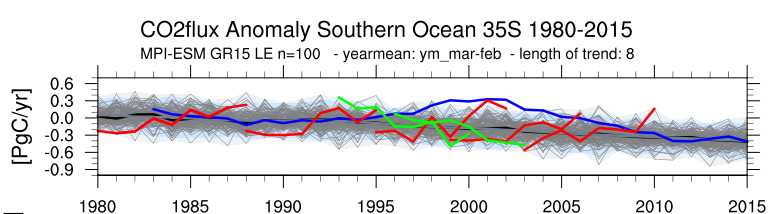
\includegraphics[scale=.78]{SOCS.png}
\label{fig:evolution_southern_ocean_carbon_sink}
\caption{Evolution of the Southern Ocean carbon sink anomaly south of 35°S. Grey lines show the 100 ensemble members, the black line the ensemble median, the gray shading is the range of the ensemble, the blue shading is the 2σ ensemble spread, the red lines are decreasing sink trend candidates, the green line increasing sink trend candidates, the blue line is the SOM-FFN observation-based estimate}
\end{figure}

As an entry point of our analysis, we try to find trends similar to the anomalous outgassing trends of SOM-FFN data from the 1990s. To get a large sample size, we take running interval boundaries. Because of the overestimated seasonal cycle of primary production in HAMOCC \cite{Nevison2016}, we compute trends of the annual Southern Ocean Carbon trend. The amount of trends and the corresponding significance vary depending on the choosen length of trends (SI Fig.1 Trend Heatmap). A monotonous trend of ten years only appears once in 2600 available intervals. Most continuous trends only sustain for shorter than a decade. To ensure a certain amount of monotonous trends and a similar trendlength to a decade, we take 8-year trends in this analysis. For a meaningful analysis of the impact of biology, we separate the years in March to February [CHANGE THIS TO JUNE-MAY ONCE NEW FIGURES APPEAR] , to ensure that a complete primary production bloom is captured in each year. Furthermore, the members used in this study are required to be monotonous similar to SOM-FFN data in the 1990s.
 
Applying those requirements, we find three candidates of decreasing decadal trend. They appear independent of the timestamp in the simulation, although increasing atmospheric pCO2 forcing would favor earlier decades. These candidates are mostly in the 2σ ensemble spread. 


\section{Results II: Spatial distribution of Southern Ocean carbon sink trend}

The Southern ocean shows zonal structures in variables related to the carbon sink. 
The large member ensemble mean is defined as the ‘forced’ signal, and the differences of single members with the ensemble mean as standard deviation equals internal variability, respectively \cite{Deser2012}. The ‘forced’ signals in the Southern Ocean show dominant increasing trend (Fig. \ref{fig:SOCS_ensmean_ensstd} left). Also in spatial distribution, the carbon sink in each grid point follows a normal distribution (Fig. \ref{fig:SOCS_spatial_gaussian}). The standard deviation (Fig. \ref{fig:SOCS_ensmean_ensstd} right) shows differences in magnitude of internal variability in a zonal pattern. The largest internal variability appears in 50-60$^\circ$S south of the polar front, where outgassing occurs. Internal variability seems to drop north of 45$^\circ$S, showing the large internal variability of the Southern Ocean compared to other basins.

\begin{figure}
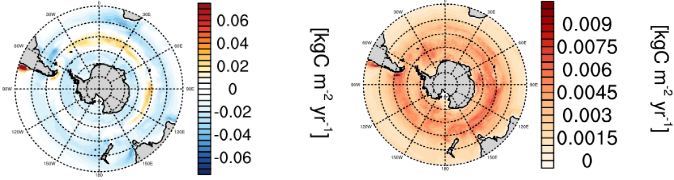
\includegraphics[scale=.9]{SOCS_ensmean_ensstd.png} % from gfx folder
\label{fig:SOCS_ensmean_ensstd}
\caption{Southern Ocean carbon sink (20-year mean): ensemble median (left) as forced signal and ensemble standard deviation (right) as internal variability [SHOULD I INCLUDE THE SAME FOR INTPP???]}
\end{figure}

Exemplarily for all decadal decreasing carbon sink trend members, we show the candidate of most extreme case of anomalous outgassing. The region of 50-60$^\circ$S has the strongest decreasing trend in CO$_2$flux.

As shown in previous studies \cite{LeQuere2007}, the variations of oceanic carbon uptake are related to the background thermal and dynamic changes. Insight to the drivers is gained by separating the pCO$_2$ seasonal amplitude in a component driven by changes in sea surface temperature (the thermal trend; Fig. SI \ref{fig:dpco2_separation}) and one driven by changes in DIC and/or alkalinity (the non-thermal trend: Fig. SI \ref{fig:dpco2_separation}) \cite{Takahashi2002}. The non-thermal trend dominates the seasonal amplitude and decreases in 50-60$^\circ$S.


\begin{figure}
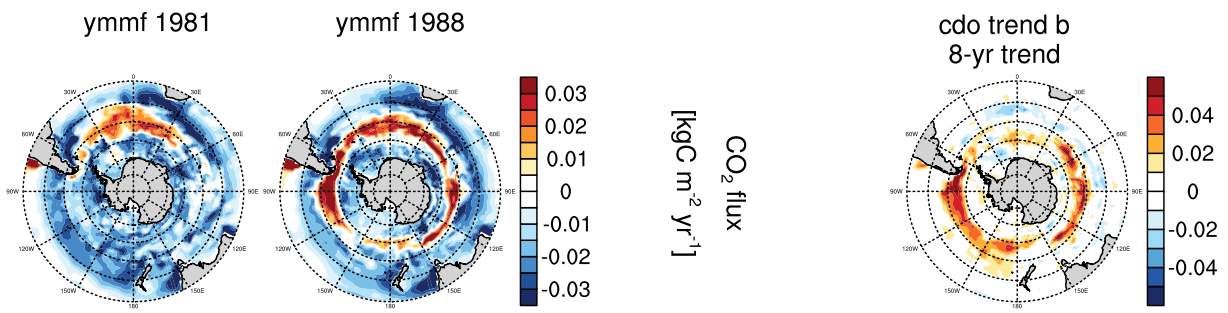
\includegraphics[scale=.35]{co2flux.png} % from gfx folder
\label{fig:co2flux}
\caption{CO$_2$flux in the first and last year of the trend period; trend over 8 years}
\end{figure}


\begin{figure}
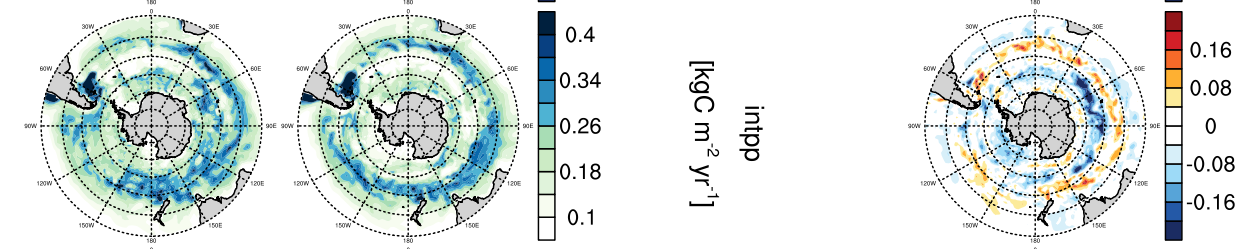
\includegraphics[scale=.35]{intpp.png} % from gfx folder
\label{fig:intpp}
\caption{Vertically integrated primary production in the first and last year of the trend period; trend over 8 years}
\end{figure}

Primary production and CO$_2$flux show opposing trends as plankton growth takes up large amounts of surface DIC and hence lowers pCO$_2$ each season. 
Temperature, nutrients and light availability can directly effect the phytoplankton growth rate. But there are no significant trends detected south of 40$^\circ$S. The Southern Ocean as an upwelling area has plenty of supply of nutrients from below. Even in the austral summer months, the nutrient limitation function stays close to 1, which mean not limiting at all. Nutrient concentrations in surface nitrate, phosphate or iron also follow the opposite path of primary produce: They have an increasing trend where less consequently less primary production declined over the trend period. Contrary, in region of increased primary production, nutrient concentrations decreased. Therefore we conclude that in our model the southern ocean is not nutrient depleted. Hence the probable increase of upwelling deep ocean nutrients effects the primary production little.

\begin{figure}
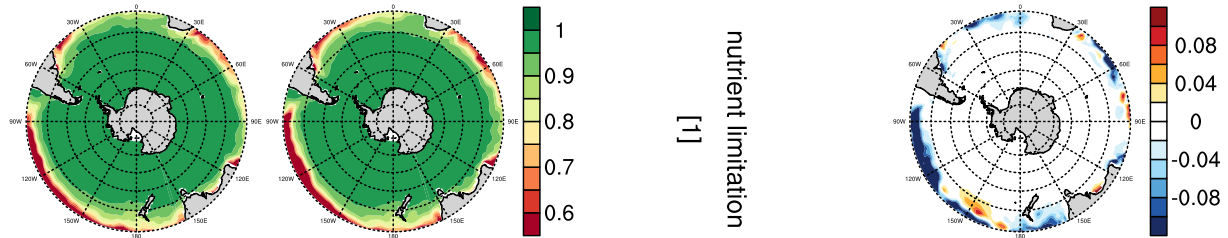
\includegraphics[scale=.5]{nutrient_limitation.png} % from gfx folder
\label{fig:nutrient_limitation}
\caption{Nutrient limitation for primary production in the first and last year of the trend period; trend over 8 years}
\end{figure}


However there seems to be a deeper mixed depth layer in 50$^\circ$S. Mixing can bring phytoplankton to deeper depths where the are exposed to less light which inhibits growth. Sverdrup \cite{Sverdrup1953} introduced his concept of critical depth based turbulent mixing \cite{Franks2014} as a requirement for plankton blooms. We use his theory not in an overall manner discussing plankton bloom dynamics, but rather the straight-forward effect of mixing of plankton to deeper layers. 
Sverdrup based this theory on turbulent mixing. However here we use a hydrologically mixed layer depth based on a density criterion which serves as a first approach to wind-induced mixing strength. 

\begin{figure}
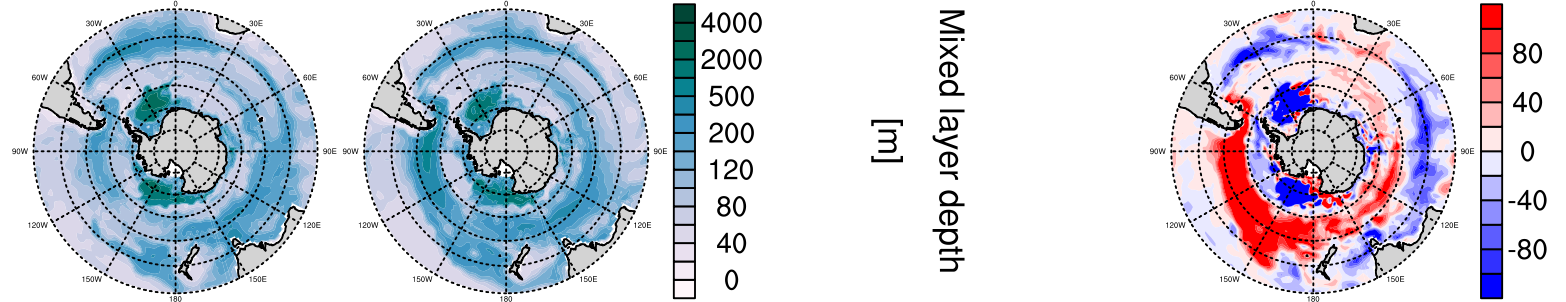
\includegraphics[scale=.4]{zmld.png} % from gfx folder
\label{fig:zmld}
\caption{Mixed depth layer in the first and last year of the trend period; trend over 8 years}
\end{figure}

To visualize mixing of phytoplankton towards deeper layers, we calculated an average depth of phytoplankton mass based on the mechanics of centre of mass. Here we see an increase in depth in the 50s$^\circ$S indicating deeper mixing and hence less light availability. At 50-60$^\circ$S we see a 3m drop of plankton average depth from 22m to 25m. This change in depth is accompanied by a decrease of ~10\% in solar radiation. As primary production is a highly non-linear process, this lower growth rate drastically impacts the plankton bloom.


Deeper winter mixing also effects the plankton bloom as it shortens the available time of a stratified water column required for primary production. The water columns of the Southern Ocean are deeperly mixed in the winter seasons. In spring, solar radiation restratifies the water column. The more mixing happened in winter and during restratification spring, the longer plankton cannot bloom. So wind-mixing has a two-fold implication on primary production and the carbon sink: It shortens the timeframe for primary production and it deepens a fraction of the standing stock.

\begin{figure}
%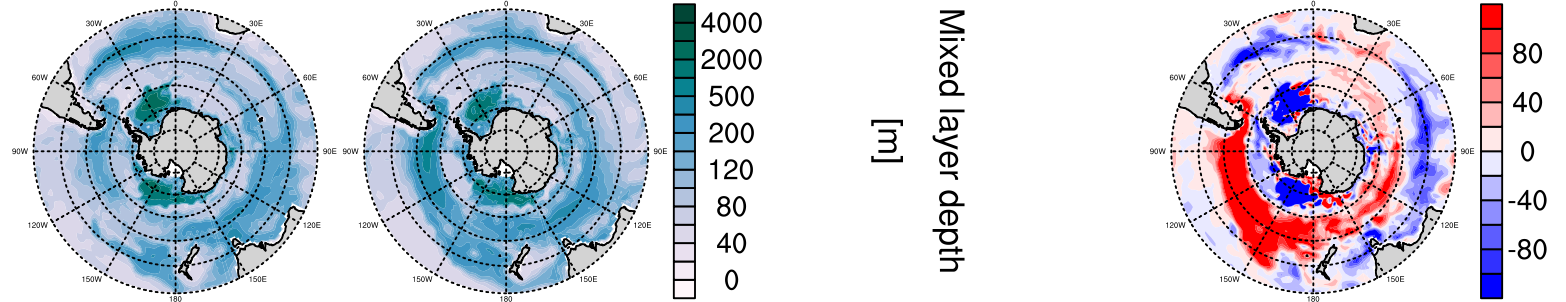
\includegraphics[scale=.4]{zmld.png} % from gfx folder
\label{fig:zmld_intpp_seasonality}
\caption{Changes on the seasonality of vertically integrated primary production and mixed depth layer {MISSING}}
\end{figure}


Previous studies state that intensified wind lead to increased upwelling, which then impacts the surface pCO$_2$ to rise and thereby weaken the carbon uptake. Our candidates also show this pattern: Intensified winds (Fig. \ref{fig:slp_wind}) are reflected in increased trend in SAM (Fig. SI). 

Increased upwelling lowers sea-surface temperature and thereby lowers stratification, so wind stress is more easily mixing the water column.

\begin{figure}
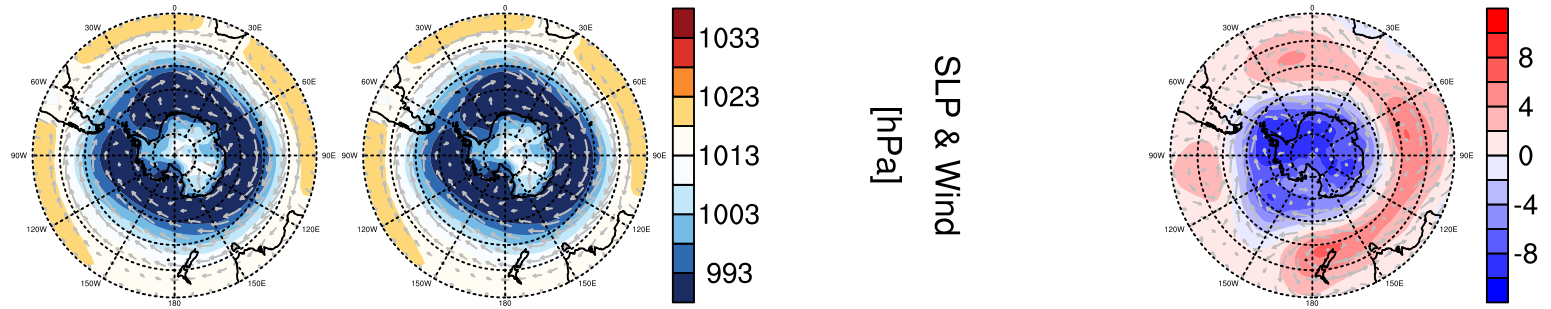
\includegraphics[scale=.4]{slp_wind.png} % from gfx folder
\label{fig:slp_wind}
\caption{Sea-level pressure and wind fields in the first and last year of the trend period; trend over 8 years}
\end{figure}

We reason that intensified winds cause increased turbulent mixing of the water column (Fig. \ref{fig:wind_mixing}). Deeper mixing occurs in 50-60$^\circ$S whereas 40-50$^\circ$S experiences less winds stabilizing the water column.

\begin{figure}
%\includegraphics[scale=.4]{wind_mixing.png} % from gfx folder
\label{fig:wind_mixing}
\caption{Vertical diffusivity due to wind in the first and last year of the trend period; trend over 8 years}
\end{figure}


We were not able to attribute weights on the two follow-up effects on upwelling in the sense of impact on the carbon sink.



\section{Discussion}
Lovenduski and Gruber 2005: how is model different, how are results different
\begin{enumerate}
\item increase in SAM → increase in chlorophyll south of PF/45°S because of iron supply from below (we have decrease)
\item increase in SAM→ reduction in chlorophyll north of PF/45°S because of increased ZMLD
\item BUT we dont have iron limitation in SO
\end{enumerate} 

Limitations of HAMOCC vs obs:
\begin{enumerate}
\item seasonal cycle \cite{Nevison2016}
\item location of polar yet in ECHAM
\item basically no nutrient limitation in SO? - other models and obs disagree
\item observations also sparse (mostly cruises) or proxy satelite chl-a
\item MPIOM performance on circulation patterns and water masses (Yohei mentioned Anne M. could know this) in SO
\item only one phytoplankton type in HAMOCC? - some models have more
\end{enumerate} 



\section{Summary and conclusions}

MPI-ESM large ensemble simulations produces internal variability of the Southern Ocean carbon sink including decreasing decadal carbon sink trends over the past decades, which were seen in observations. Decreasing carbon sink trends were accompanied by increasing trends of the Southern Annular Mode on the Southern Ocean carbon sink as in \cite{LeQuere2007}. The results winds not only enhance upwelling of carbon-rich waters, but also change water column stability which let primary production to overall decrease and to shift northwards. Over all the Southern Ocean, biology decreases in a negative trend of the Southern Ocean carbon sink. 

\section*{Acknowledgements}
Thanks to Luis Kornblueh, Jürgen Kröger, Michael Botzet for making the large ensemble simulations available. The simulations were performed at the Swiss national supercomputing center (CSCS) and the German Climate Computing Center (DKRZ). Primary data and scripts used in the analysis of this study are archived by the Max Planck Institute for Meteorology and can be obtained by contacting publications@mpimet.mpg.de.


\newpage

\bibliography{SouthernOceanCarbonSink_new}

\bibliographystyle{Science}

\newpage

\section*{Supplementary information}

\subsection*{Normal distributions of the southern ocean carbon sink}
\begin{figure}
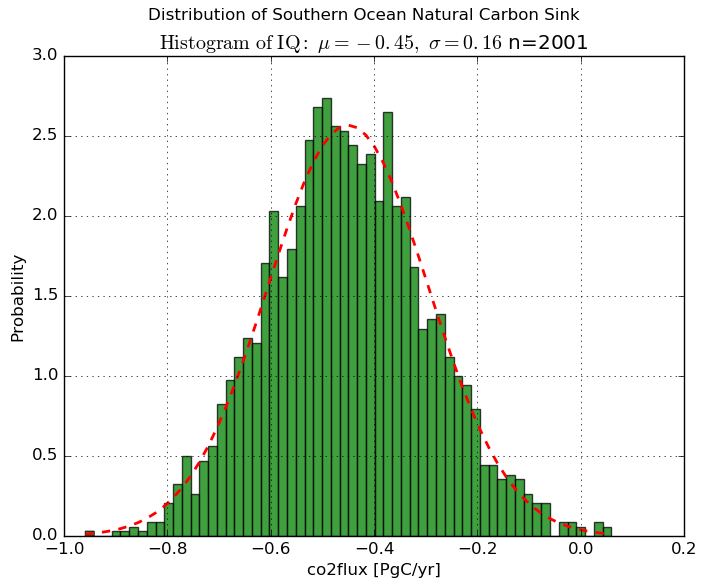
\includegraphics[scale=.5]{SOCS_temporal_gaussian.png} % from gfx folder
\label{fig:SOCS_temporal_gaussian}
\caption{Southern Ocean carbon sink fieldsum 35-90S}
\end{figure}

\begin{figure}
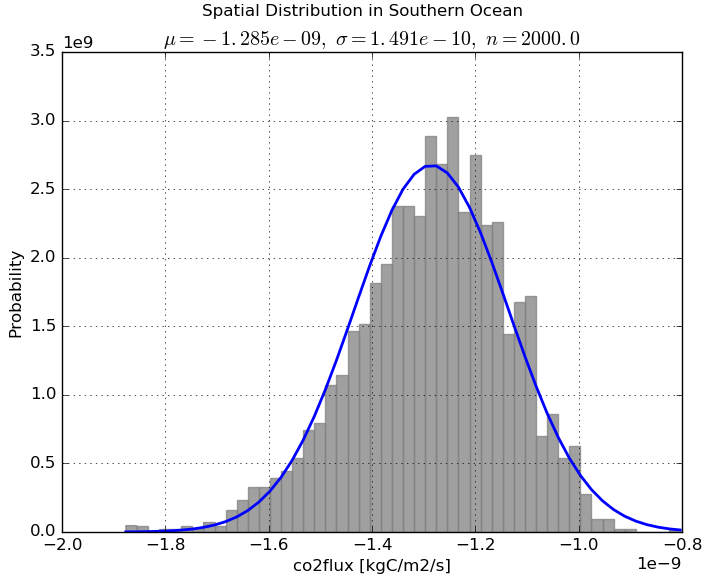
\includegraphics[scale=.5]{SOCS_spatial_gaussian.png} % from gfx folder
\label{fig:SOCS_spatial_gaussian}
\caption{Southern Ocean carbon sink for a random gridpoint in the Southern Ocean}
\end{figure}

\subsection*{Delta pCO$_2$-separation}
\begin{figure}
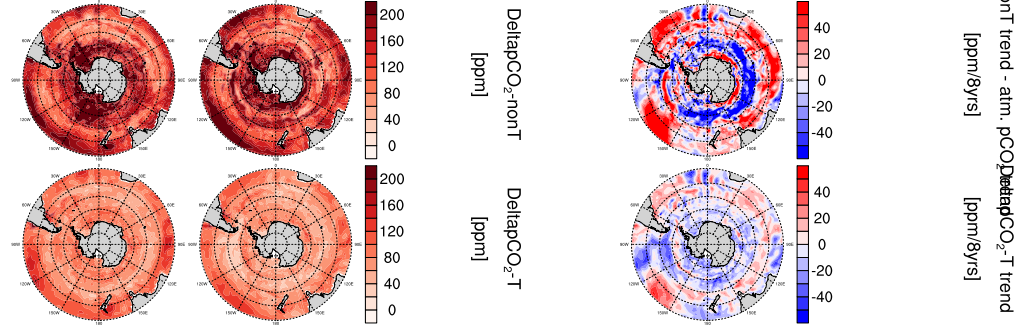
\includegraphics[scale=.6]{dpco2_separation.png} % from gfx folder
\label{fig:dpco2_separation}
\caption{Delta pCO$_2$-separation \cite{Takahashi2002}}
\end{figure}

%\begin{figure}
%\includegraphics[scale=1]{.png} % from gfx folder
%\label{fig:title}
%\caption{something}
%\end{figure}

\subsection*{Selection criteria for decadal trend members}
\begin{enumerate}
\item positive CO2flux trend: value PgC/yr
\item monotony Mann-Kendall
\item significance student t-Test
\end{enumerate}

\newpage

\newpage

\newpage

\section*{Formatting Citations}

Citations can be handled in one of three ways.  The most
straightforward (albeit labor-intensive) would be to hardwire your
citations into your \LaTeX\ source, as you would if you were using an
ordinary word processor.  Thus, your code might look something like
this:


\begin{quote}
\begin{verbatim}
However, this record of the solar nebula may have been
partly erased by the complex history of the meteorite
parent bodies, which includes collision-induced shock,
thermal metamorphism, and aqueous alteration
({\it 1, 2, 5--7\/}).
\end{verbatim}
\end{quote}


\noindent Compiled, the last two lines of the code above, of course, would give notecalls in {\it Science\/} style:

\begin{quote}
\ldots thermal metamorphism, and aqueous alteration ({\it 1, 2, 5--7\/}).
\end{quote}

Under the same logic, the author could set up his or her reference list as a simple enumeration,

\begin{quote}
\begin{verbatim}
{\bf References and Notes}

\begin{enumerate}
\item G. Gamow, {\it The Constitution of Atomic Nuclei
and Radioactivity\/} (Oxford Univ. Press, New York, 1931).
\item W. Heisenberg and W. Pauli, {\it Zeitschr.\ f.\ 
Physik\/} {\bf 56}, 1 (1929).
\end{enumerate}
\end{verbatim}
\end{quote}

\noindent yielding

\begin{quote}
{\bf References and Notes}

\begin{enumerate}
\item G. Gamow, {\it The Constitution of Atomic Nuclei and
Radioactivity\/} (Oxford Univ. Press, New York, 1931).
\item W. Heisenberg and W. Pauli, {\it Zeitschr.\ f.\ Physik} {\bf 56},
1 (1929).
\end{enumerate}
\end{quote}

That's not a solution that's likely to appeal to everyone, however ---
especially not to users of B{\small{IB}}\TeX\   If you
are a B{\small{IB}}\TeX\ user, we suggest that you use the
\texttt{Science.bst} bibliography style file and the
\texttt{scicite.sty} package, both of which we are downloadable from our author help site
(http://www.sciencemag.org/about/authors/prep/TeX\_help/).  You can also
generate your reference lists by using the list environment
\texttt{\{thebibliography\}} at the end of your source document; here
again, you may find the \texttt{scicite.sty} file useful.

Whether you use B{\small{IB}}\TeX\ or \texttt{\{thebibliography\}}, be
very careful about how you set up your in-text reference calls and
notecalls.  In particular, observe the following requirements:

\begin{enumerate}
\item Please follow the style for references outlined at our author
  help site and embodied in recent issues of {\it Science}.  Each
  citation number should refer to a single reference; please do not
  concatenate several references under a single number.
\item Please cite your references and notes in text {\it only\/} using
  the standard \LaTeX\ \verb+\cite+ command, not another command
  driven by outside macros.
\item Please separate multiple citations within a single \verb+\cite+
  command using commas only; there should be {\it no space\/}
  between reference keynames.  That is, if you are citing two
  papers whose bibliography keys are \texttt{keyname1} and
  \texttt{keyname2}, the in-text cite should read
  \verb+\cite{keyname1,keyname2}+, {\it not\/}
  \verb+\cite{keyname1, keyname2}+.
\end{enumerate}

\noindent Failure to follow these guidelines could lead
to the omission of the references in an accepted paper when the source
file is translated to Word via HTML.

\section*{Handling Math, Tables, and Figures}

Following are a few things to keep in mind in coding equations,
tables, and figures for submission to {\it Science}.

\paragraph*{In-line math.}  The utility that we use for converting
from \LaTeX\ to HTML handles in-line math relatively well.  It is best
to avoid using built-up fractions in in-line equations, and going for
the more boring ``slash'' presentation whenever possible --- that is,
for \verb+$a/b$+ (which comes out as $a/b$) rather than
\verb+$\frac{a}{b}$+ (which compiles as $\frac{a}{b}$).  Likewise,
HTML isn't tooled to handle certain overaccented special characters
in-line; for $\hat{\alpha}$ (coded \verb+$\hat{\alpha}$+), for
example, the HTML translation code will return [\^{}$(\alpha)$].
Don't drive yourself crazy --- but if it's possible to avoid such
constructs, please do so.  Please do not code arrays or matrices as
in-line math; display them instead.  And please keep your coding as
\TeX-y as possible --- avoid using specialized math macro packages
like \texttt{amstex.sty}.

\paragraph*{Displayed math.} Our HTML converter sets up \TeX\
displayed equations using nested HTML tables.  That works well for an
HTML presentation, but Word chokes when it comes across a nested
table in an HTML file.  We surmount that problem by simply cutting the
displayed equations out of the HTML before it's imported into Word,
and then replacing them in the Word document using either images or
equations generated by a Word equation editor.  Strictly speaking,
this procedure doesn't bear on how you should prepare your manuscript
--- although, for reasons best consigned to a note, we'd
prefer that you use native \TeX\ commands within displayed-math
environments, rather than \LaTeX\ sub-environments.

\paragraph*{Tables.}  The HTML converter that we use seems to handle
reasonably well simple tables generated using the \LaTeX\
\texttt{\{tabular\}} environment.  For very complicated tables, you
may want to consider generating them in a word processing program and
including them as a separate file.

\paragraph*{Figures.}  Figure callouts within the text should not be
in the form of \LaTeX\ references, but should simply be typed in ---
that is, \verb+(Fig. 1)+ rather than \verb+\ref{fig1}+.  For the
figures themselves, treatment can differ depending on whether the
manuscript is an initial submission or a final revision for acceptance
and publication.  For an initial submission and review copy, you can
use the \LaTeX\ \verb+{figure}+ environment and the
\verb+\includegraphics+ command to include your PostScript figures at
the end of the compiled PostScript file.  For the final revision,
however, the \verb+{figure}+ environment should {\it not\/} be used;
instead, the figure captions themselves should be typed in as regular
text at the end of the source file (an example is included here), and
the figures should be uploaded separately according to the Art
Department's instructions.


\section*{What to Send In}

What you should send to {\it Science\/} will depend on the stage your manuscript is in:

\begin{itemize}
\item {\bf Important:} If you're sending in the initial submission of
  your manuscript (that is, the copy for evaluation and peer review),
  please send in {\it only\/} a PostScript or PDF version of the
  compiled file (including figures).  Please do not send in the \TeX\ 
  source, \texttt{.sty}, \texttt{.bbl}, or other associated files with
  your initial submission.  (For more information, please see the
  instructions at our Web submission site,
  http://www.submit2science.org/ .)
\item When the time comes for you to send in your revised final
  manuscript (i.e., after peer review), we require that you include
  all source files and generated files in your upload.  Thus, if the
  name of your main source document is \texttt{ltxfile.tex}, you
  need to include:
\begin{itemize}
\item \texttt{ltxfile.tex}.
\item \texttt{ltxfile.aux}, the auxilliary file generated by the
  compilation.
\item A PostScript file (compiled using \texttt{dvips} or some other
  driver) of the \texttt{.dvi} file generated from
  \texttt{ltxfile.tex}, or a PDF file distilled from that
  PostScript.  You do not need to include the actual \texttt{.dvi}
  file in your upload.
\item From B{\small{IB}}\TeX\ users, your bibliography (\texttt{.bib})
  file, {\it and\/} the generated file \texttt{ltxfile.bbl} created
  when you run B{\small{IB}}\TeX.
\item Any additional \texttt{.sty} and \texttt{.bst} files called by
  the source code (though, for reasons noted earlier, we {\it
    strongly\/} discourage the use of such files beyond those
  mentioned in this document).
\end{itemize}
\end{itemize}

% Your references go at the end of the main text, and before the
% figures.  For this document we've used BibTeX, the .bib file
% scibib.bib, and the .bst file Science.bst.  The package scicite.sty
% was included to format the reference numbers according to *Science*
% style.


%\bibliography{SouthernOceanCarbonSink_new}

%\bibliographystyle{Science}



% Following is a new environment, {scilastnote}, that's defined in the
% preamble and that allows authors to add a reference at the end of the
% list that's not signaled in the text; such references are used in
% *Science* for acknowledgments of funding, help, etc.

\begin{scilastnote}
\item We've included in the template file \texttt{scifile.tex} a new
environment, \texttt{\{scilastnote\}}, that generates a numbered final
citation without a corresponding signal in the text.  This environment
can be used to generate a final numbered reference containing
acknowledgments, sources of funding, and the like, per {\it Science\/}
style.
\end{scilastnote}




% For your review copy (i.e., the file you initially send in for
% evaluation), you can use the {figure} environment and the
% \includegraphics command to stream your figures into the text, placing
% all figures at the end.  For the final, revised manuscript for
% acceptance and production, however, PostScript or other graphics
% should not be streamed into your compliled file.  Instead, set
% captions as simple paragraphs (with a \noindent tag), setting them
% off from the rest of the text with a \clearpage as shown  below, and
% submit figures as separate files according to the Art Department's
% instructions.


\clearpage

\noindent {\bf Fig. 1.} Please do not use figure environments to set
up your figures in the final (post-peer-review) draft, do not include graphics in your
source code, and do not cite figures in the text using \LaTeX\
\verb+\ref+ commands.  Instead, simply refer to the figure numbers in
the text per {\it Science\/} style, and include the list of captions at
the end of the document, coded as ordinary paragraphs as shown in the
\texttt{scifile.tex} template file.  Your actual figure files should
be submitted separately.



\end{document}




















